\documentclass[10pt]{beamer}

%% Chinese support
%% \usepackage[adobefonts,nocap]{ctex}

%% Fonts
\usepackage{multicol}
\usepackage{mathabx}
\usepackage[scaled]{helvet}
\usepackage{lmodern}
\usepackage{eulervm}
\usefonttheme[onlymath]{serif}
\usefonttheme{professionalfonts}
\usefonttheme{structurebold}
\usepackage{bm}
\hypersetup{
  colorlinks=true,
  linkcolor=blue,
  citecolor=blue,
  urlcolor=blue}

%% Color & Theme
\definecolor{SUblue}{RGB}{0,0,180}
\usecolortheme[RGB={0,0,180}]{structure}
\usetheme{Boadilla}
\setbeamertemplate{navigation symbols}{}
\setbeamertemplate{itemize items}[circle]
\setbeamertemplate{enumerate items}[circle]
\setbeamerfont{title}{size=\large}
\setbeamerfont{frametitle}{size=\large}
\setbeamerfont{framesubtitle}{size=\large,shape =$\color{violet}{\looparrowdownright}~$}
\setbeamercolor{title}{fg=white, bg= SUblue!75!green}
\setbeamercolor{framesubtitle}{fg=violet}
%\setlength{\leftmargini}{5pt}


\title[Statistical Computing]{{\textbf{Statistical Computing: Introduction}}}

\author[Feng Li]{
\includegraphics[height=2cm]{cufelogo}\\
  \vspace{0.5cm}\textbf{Feng Li\\\texttt{feng.li@cufe.edu.cn}}}
\date{}
\institute[Stat \& Math, CUFE]{\footnotesize{\textbf{School of Statistics and
      Mathematics\\ Central University of Finance and Economics}}}

%%%%%%%%%%%%%%%%%%%%%%%%%%%%%%%%%%%%%%%%%%%%%%%%%%%%%%%%%%%%%%%%%%%%%%%%%%%%%%%
\begin{document}

%% Title page
\begin{frame}[plain]
  \titlepage
  \tiny{Revised on \today}
\end{frame}


\section{General information}
\begin{frame}
  \frametitle{General information}
  \begin{itemize}

  \item \textbf{Lecturer}

    \begin{itemize}
    \item Feng Li, \texttt{feng.li@cufe.edu.cn}
    % \item Anastasios Panagiotelis, \texttt{anastasios.panagiotelis@monash.edu}
    \end{itemize}
  \item \textbf{Language}: The course is taught in Chinese. The course
    materials are in English. %And all the assignments and examinations will be
    %conducted in English.

  \item \textbf{Reception hours}: Questions concerned with this course can be
    asked after each lecture or via email.

  \item \textbf{Lecture notes and course materials}

    \begin{itemize}

    \item \textbf{An Introduction to R} (\texttt{http://cran.r-project.org/doc/manuals/R-intro.pdf})

    \item \textbf{Introduction to Scientific Programming and Simulation Using R} by Owen
      Jones, Robert Maillardet, Andrew Robinson

    \item Course materials and updated news are available at the course homepage
      \texttt{(http://feng.li/teaching/statcomp/)}

    \end{itemize}


  \item \textbf{Working load}: Depending on your own situation and you
    ambition, you decide how much time you want to input. But there are
    compulsory assignments including presentation and discussions should be
    done in order to pass the exam.

  \end{itemize}
\end{frame}

\begin{frame}
\frametitle{Assignments and examinations}

To pass the final exam you have to have at least 60p in the total score with
the following tasks.

  \begin{itemize}
  \item \textbf{Lab assignments and presentation} (50\%)

    % There will be a \textbf{mandatory} presentation (30p) for each of you.

  \item \textbf{Computer-based examinations} (50\%)

 \end{itemize}
\end{frame}

\begin{frame}[plain]
  \addtocounter{framenumber}{-1}
  \begin{center}
    {\color{SUblue} \textbf{\Huge Don't worry and it's fun!}}
  \end{center}
\end{frame}


\begin{frame}
  \frametitle{The Evolution of Statistical Computing}

  \begin{figure}
    \centering
    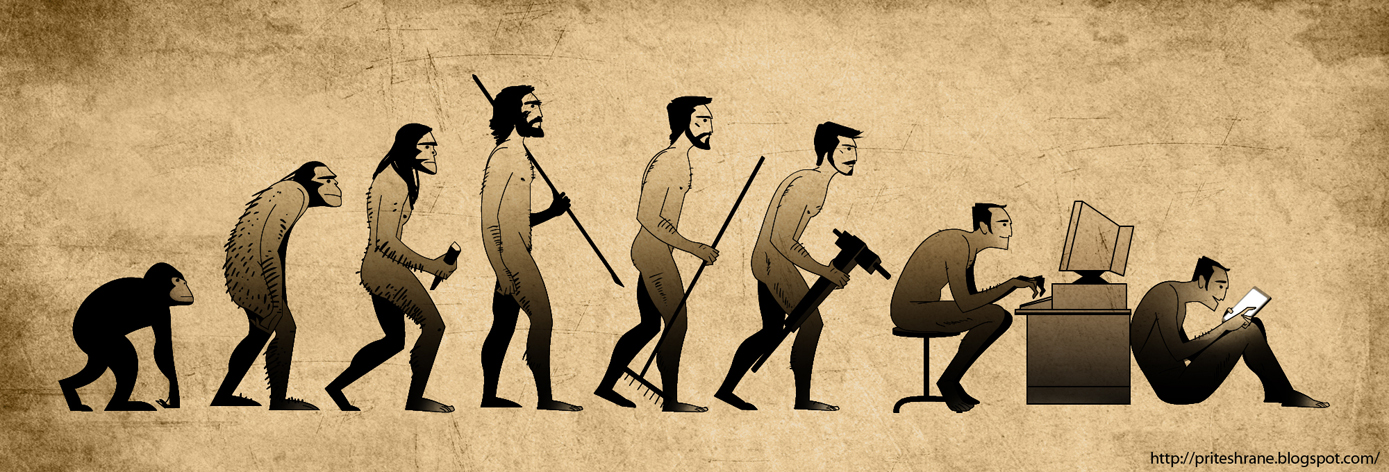
\includegraphics[width=\textwidth]{evolution}
  \end{figure}

\end{frame}


\begin{frame}
  \frametitle{The R programing language}

  \begin{itemize}
  \item R is an implementation of the S programming language inspired by Scheme.

  \item S was created by John Chambers while at Bell Labs in the 70's.

  \item Up to that time, much of the statistical computing was done by directly
    calling Fortran subroutines; however, S was designed to offer an alternate
    and more interactive approach.

  \item R was created by Ross Ihaka and Robert Gentleman at the University of
    Auckland, New Zealand.

  \item R is named partly after the first names of the first two R authors and
    partly as a play on the name of S.

  \item R is currently developed by the R Development Core
    Team, of which Chambers is a member.

  \item R is the top statistical language in the TIOBE index which is also
    above the commercial software SAS.

  \item R can be easily used in Big Data analysis platforms, e.g. Hadoop/Spark.

  \end{itemize}
\end{frame}


\begin{frame}
\frametitle{Installing R}
Installing \textbf{R} on your own computer is simple and free.
\begin{enumerate}
\item If you use Microsoft Windows, visit
  \url{http://www.r-project.org/}. It shipped with a simple graphical user
  interface (GUI).

\item R is available for Mac OS X users with a nice build-in graphical user
  interface, visit \url{http://www.r-project.org}

\item If you use Linux, search the phrase ``r-cran'' in your system's software
  repository. Any text editor can be used to edit R source code. But if you
  want a graphical user interface, \textbf{RStudio} (with is easy to install and also
  available for other platforms) is a good start. Please visit
  \url{http://www.rstudio.org/download/desktop}.
\end{enumerate}
\end{frame}


\begin{frame}
  \frametitle{Suggested reading}

  \begin{itemize}
  \item R-intro: \textbf{Chapter 1, Appendix B, C}
  \end{itemize}

\end{frame}


\end{document}
